\documentclass{article}
\usepackage{graphicx}
\usepackage[a4paper, margin=2cm]{geometry}
\usepackage{wrapfig}
\usepackage{hyperref} % Add this line
\usepackage{tabulary}
\usepackage{multicol}
\usepackage{array}

\title{University of Moratuwa\\
    Department of Electronic and Telecommunication Engineering\\}

\begin{document}

\maketitle

\vspace{5pt}

\begin{center}
	
\includegraphics[width=0.5\textwidth]{University_of_Moratuwa_logo.png}
	\\
	\LARGE EN2031 - Fundamentals of Computer Organization and Design
	\\
	\vspace{5pt}
	{Motherboard Dissection Report}\\
	{Team Ciscers-Riscers}
\end{center}

\begin{center}
	\vspace{0.5cm} % Adds space between heading and table
	\renewcommand{\arraystretch}{2} % Increases row height
	\begin{tabular}{|c|c|c|}
		\hline
		\multicolumn{3}{|c|}{\textbf{Group Members}} \\
		\hline
		\textbf{Index Number} & \textbf{Name}  &\textbf{Tasks allocation}  \\
		\hline
		220212A      & Hapuarachchi HADND  & \\
		\hline
		220212A      & Gunathilaka K.L.   & \\
		\hline
		220212A      & Hapuarachchi HADND & \\
		\hline
	\end{tabular}
\end{center}

\newpage

\tableofcontents

\section{Abstract}
\fontsize{12pt}{13pt}\selectfont
Our dissection report is based on the MSI B460M PRO-VDH WIFI motherboard
and the main inceptions are Identification of main components and their
key specifications, Cooling Options, Connectivity options with their key
specifications, IO component classification based on their access speeds,
and Functional Block Diagram indicating all the main components and their
inter-connectivity.

\section{Introduction}

One of the standout features of this motherboard is its integrated Wi-Fi 6
technology, which offers faster and more reliable wireless connectivity
compared to previous generations. This makes it an excellent choice for
users who require stable internet connections for gaming, streaming, or
professional work. Additionally, the motherboard includes a variety of
connectivity options such as USB 3.2 Gen 1 ports, HDMI, and DisplayPort
outputs, ensuring compatibility with a wide range of peripherals and displays.
The B460M PRO-VDH WIFI also emphasizes cooling and thermal management,
featuring multiple fan headers and comprehensive controls via the MSI Dragon
Center software. This allows users to optimize their cooling setup to maintain
optimal temperatures under various workloads. The motherboard's layout is
designed to facilitate easy installation and upgrades, with ample space for
memory modules, storage devices, and expansion cards.Furthermore, the
motherboard supports dual-channel DDR4 memory, with speeds up to 2933 MHz,
providing ample bandwidth for multitasking and demanding applications. The


\section{Motherboard Layout}
\begin{figure}[ht]
\centering
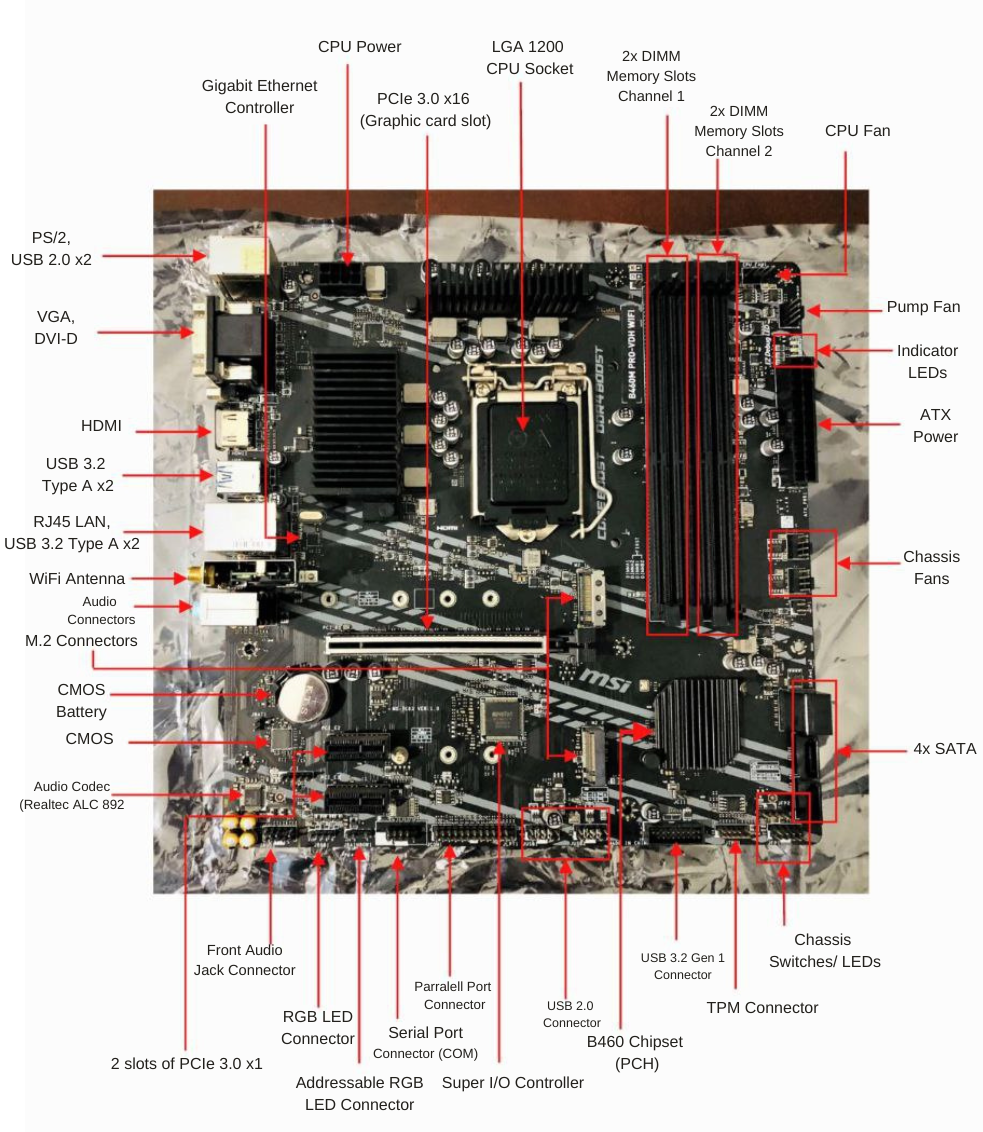
\includegraphics[height=0.95\textwidth]{overview.png}
\end{figure}

\section{Main Components}

\subsection{Processor}
\begin{wrapfigure}[11]{r}{0.28\textwidth}
	\centering
	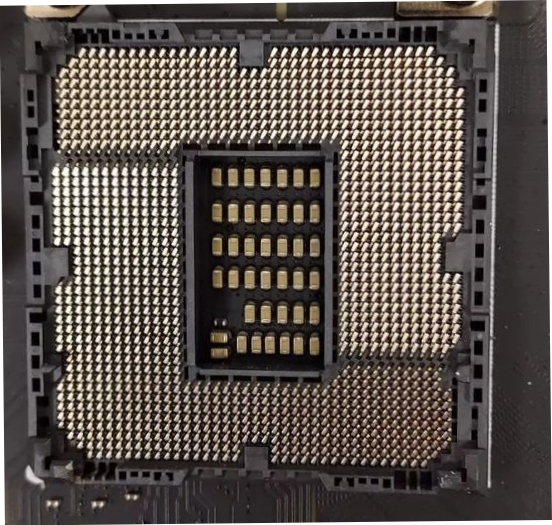
\includegraphics[width=0.25\textwidth]{socket-modified.png}
\end{wrapfigure}

MSI B460M PRO-VDH WIFI motherboard supports 10th Gen Intel Core (i3, i5, i7, i9) and
Pentium Gold / Celeron processors for LGA 1200 socket (Socket H5). Unfortunately, This
motherboard does not support overclocking (For Intel we need a Z or X series Motherboard) 
and the dissected computer had a Intel i5-10600K, which is a unlocked processor. 
\\
Processor socket allows the CPU to be mounted on the motherboard with the locking
mechanism. The socket is designed for variety of cooling solutions to be mounted on 
the processor such as full fan heat-sinks or custom pump fan cooling solutions with a
dedicated header pin. MSI software allows the user to monitor the temperature and control
the fan speed at different levels.   




\subsection{Memory (RAM)}

\begin{wrapfigure}[5]{r}{0.45\textwidth}
	\vspace{-30pt} 
	\centering
	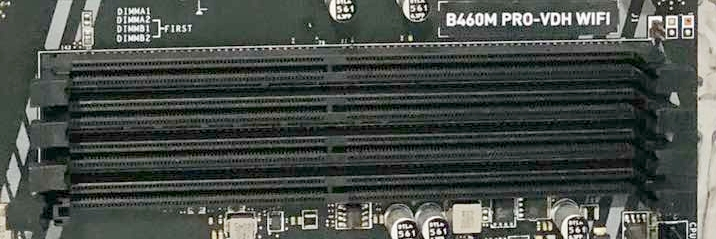
\includegraphics[width=0.45\textwidth]{ram.jpg}
\end{wrapfigure}


This motherboard features four DDR4 memory slots and maximum of 128GB 
memory. It is compatible with Intel i7 and i9 processors, supporting 2933 MHz bus speed,
and with Intel i5 and below, supporting 2666 MHz bus speed. The motherboard supports 
dual-channel mode, non-ECC(Error Correcting Code), un-buffered memory, and Intel Extreme 
Memory Profile enabled. (XMP is a memory profile that allows the user to overclock the 
 memory to higher speeds).


\subsection{Super I/O Controller}

\begin{wrapfigure}[10]{r}{0.3\textwidth}
	\centering
	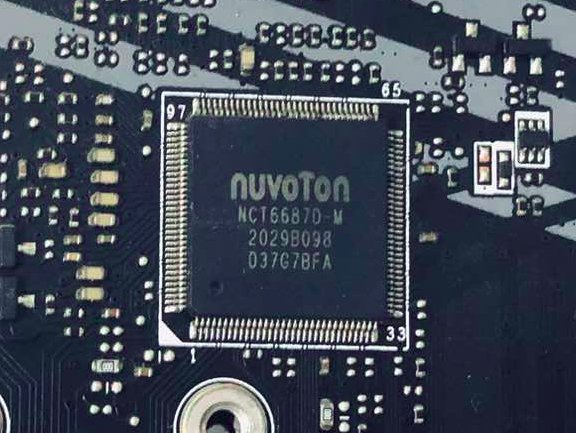
\includegraphics[width=0.3\textwidth]{nuvoton.jpg}
\end{wrapfigure}


The motherboard includes an I/O controller (NUVOTON NCT6687D Controller Chip), which
manages the input and output connections on the motherboard. The I/O controller provides
a range of connectivity options, including USB ports, audio jacks, and network connections.
It also includes features such as fan control and temperature monitoring to help manage the 
system's cooling and performance.

\begin{multicols}{2}
	\begin{itemize}
		\item No of USB Ports: 12
		\item No of SATA Ports: 6
		\item No of PCIe Lanes: 16
		\item Max Display : 3
	\end{itemize}
\end{multicols}


\subsection{Storage}

\begin{wrapfigure}[8]{r}{7.5em}
	\vspace{-30pt} 
	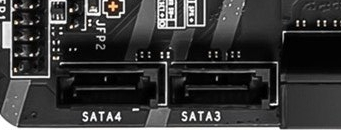
\includegraphics[width=\linewidth]{sata.jpg}
	\smallskip
	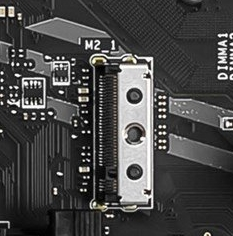
\includegraphics[width=\linewidth]{m.2.jpg}
\end{wrapfigure}
  
MSI B460M PRO-VDH WIFI motherboard supports 4 SATA ports and 2 M.2 slots for storage.
The SATA ports are used to connect traditional hard drives and solid-state drives to
the motherboard.The M.2 slots are used to connect high-speed NVMe solid-state drives,
which offer faster data transfer speeds compared to traditional SATA drives. The 
motherboard also supports RAID 0, RAID 1, RAID 5, and RAID 10 configurations. The M.2 
slots support both PCIe and SATA-based M.2 drives and very important to mention that 
the M.2 SATA SSD will disable SATA 1 port. Maximum speed of SATA is 6Gb/s and M.2 is
32Gb/s.

\subsection{Platform Controller Hub (PCH)} 
The MSI B460M PRO-VDH WIFI motherboard uses the Intel B460 chipset 
(PCH - Platform Controller Hub), which is part of Intel’s mid-range 
offering for 10th Gen Intel Core processors. This supports  up to 6 SATA ports, PCIe 3.0 lanes for expansion, 
and 12 USB ports. While it lacks overclocking capabilities (which are only 
available in Intel’s Z-series chipsets), the B460 chipset offers 
dual-channel memory support and the ability to connect various peripherals.
 It also integrates functions like Gigabit Ethernet in 
 conjunction with a dedicated Ethernet controller(Realtek RTL8111H) and other I/O management
 features to enhance system connectivity.
Additionally, the chipset handles audio I/O with the support of dedicated audio codec
like Realtek ALC892.



\section{Other Integrated Circuits}
\subsection{Ethernet Controller}

The Realtek RTL8111H IC is used to provide Gigabit LAN ethenet conenction 
to this motherboard. This supports 10/100/1000 Mbps  high speed networking 
with low latency. This also includes Green Ethernet for power-saving modes 
and support features like Wake-on-LAN(WoL), jumbo frame support, and 
hardware checksum offloading.

\subsection{Audio Codec}
\begin{wrapfigure}[7]{r}{0.15\textwidth}
	\vspace{-15pt} 
	\centering
	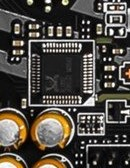
\includegraphics[width=0.15\textwidth]{audiocodec.jpg}
\end{wrapfigure}
The Realtek ALC892 is a High Definition Audio (HDA) codec chip, 
introduce 8-channel audio support, for 7.1 sound setup. It features a 
96kHz/24-bit DAC with 97db SNR and ADC with 90dB SNR for all channels. 
Also this includes line-in, line-out, mic-in, and SPDIF output options. 
Also ALC892 supports jack detection and stereo input and output re-tasking, 
along with technologies such as EAX, Dolby, and DTS for enhanced sound 
quality. This IC communicates with the PCH (Intel B460M) to provide inputs 
and outputs to both the front and back panel audio jacks.

\section{CMOS and Battery}

\begin{wrapfigure}[6]{r}{0.2\textwidth}
	\vspace{-20pt} 
	\centering
	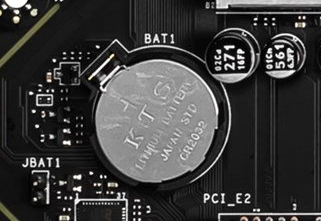
\includegraphics[width=0.2\textwidth]{cmos.jpg}
\end{wrapfigure}

CMOS stands for Complementary Metal-Oxide-Semiconductor and the main purpose is to store system 
settings, boot order and date and time. The CMOS battery is about 3V and The CMOS battery is used to 
power the CMOS chip when the computer is turned off, allowing it to retain the system settings and 
other information. If we remove it and put it back, the system will reset to default settings.


\section{Interface Standards}
\subsection{PCI (Peripheral Component Interconnect)}

Newer motherboards have PCI Express slots, which are faster than the older PCI slots. It is a
high speed serial computer expansion bus standard. It can be used to add network cards, sound
cards and graphics cards. This motherboard has 1 PCIe 3.0 x16 slots and 2 PCIe 3.0 x1 slot. The
x16 slot is used for the graphics cards ( Dissected computer had a Nvidia GTX 1660 Super graphics card.) and controlled by the CPU, and the x1 slots are used for
other expansion cards and controlled by the PCH(Platform Controller Hub).


\begin{figure}[h]
	\centering
	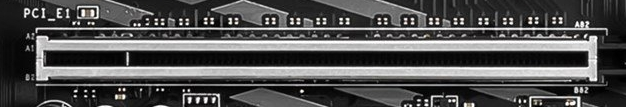
\includegraphics[width=0.5\textwidth]{pci x16.jpg}
	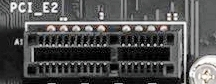
\includegraphics[width=0.3\textwidth]{pci x1.jpg}
\end{figure}


\begin{center}[h]
1x PCI-e x16 slot and 2x PCI-e x1 slots
\end{center}

\subsection{SATA}

\subsection{DMI 3.0}


\section{Functional Block Diagram}

\section{I/O Components}

\subsection{Back Panel I/O Ports}

\begin{figure}[h]
	\centering
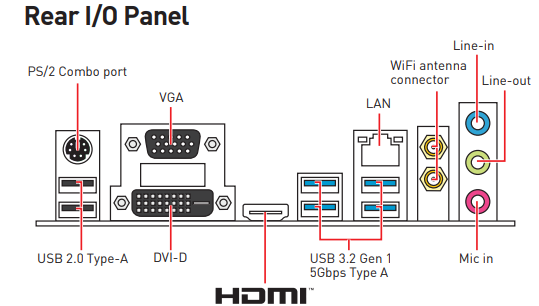
\includegraphics[width=0.8\textwidth]{backpanel.png}
\end{figure}


\subsubsection{USB}
\subsubsection{VGA}
\subsubsection{DVI}
\subsubsection{HDMI}
\subsubsection{LAN}
\subsubsection{WiFi}

\subsection{Internal Connectors}


\section{Connectivity Options}

\section{Cooling Options}



\begin{thebibliography}{9}

	\bibitem{msi} 
	MSI,"B460M PRO-VDH WIFI Motherboard Specifications", 
	\textit{MSI Official Website}. [Online]. Available: 
	\url{https://www.msi.com/Motherboard/B460M-PRO-VDH-WIFI/Specification}. [Accessed: 08-Sep-2024].
	
	\bibitem{intel} 
	Intel, "B460 Chipset", 
	\textit{Intel Official Website}. [Online]. Available: 
	\url{https://www.intel.com/content/www/us/en/products/chipsets/desktop-chipsets/b460.html}. [Accessed: 08-Sep-2024].
	
	\bibitem{realtek1}
	Realtek,"ALC892 Audio Codec Datasheet", 
	\textit{AllDatasheet.com}. [Online]. Available: 
	\url{https://www.alldatasheet.com/datasheet-pdf/pdf/1137676/REALTEK/ALC892.html}. [Accessed: 08-Sep-2024].
	
	\bibitem{realtek2}
	Realtek,"RTL8111H Datasheet", 
	\textit{AllDatasheet.com}. [Online]. Available: 
	\url{https://www.alldatasheet.com/datasheet-pdf/pdf/1253500/REALTEK/RTL8111.html}. [Accessed: 08-Sep-2024].

	\bibitem{blockDiagram}
	Forum, "Motherboard Schematic",
	\textit{elvikom.pl}.[Online]. Available:
	\url{https://www.elvikom.pl/schemat-msi-b460m-pro-vdh-wifi-ms-7c83-t67796.html}

	\bibitem{ddc}
	Wikipedia, "Display Data Channel",
	\textit{Wikipedia.com}.[Online]. Available:
	\url{https://en.wikipedia.org/wiki/Display_Data_Channel}

\end{thebibliography}
	

\end{document}